\documentclass[12pt,a4paper]{article}

\usepackage[utf8]{inputenc}
\usepackage[T1]{fontenc}
\usepackage[spanish]{babel}
\usepackage{geometry}
\usepackage{listings}
\usepackage{xcolor}
\usepackage[hidelinks]{hyperref}   
\usepackage{setspace}
\usepackage{fancyhdr}
\usepackage{parskip}
\usepackage{titlesec}
\usepackage{enumitem}
\usepackage{amsmath}
\usepackage{graphicx}
\usepackage{float}

\geometry{top=2.5cm, bottom=2.5cm, left=3cm, right=2.5cm}
\onehalfspacing

\definecolor{codegreen}{rgb}{0,0.6,0}
\definecolor{codegray}{rgb}{0.5,0.5,0.5}
\definecolor{codepurple}{rgb}{0.45,0,0.75}
\definecolor{backcolour}{rgb}{0.96,0.96,0.94}

\lstdefinestyle{pythonstyle}{
    backgroundcolor=\color{backcolour},
    commentstyle=\color{codegreen}\itshape,
    keywordstyle=\color{codepurple}\bfseries,
    stringstyle=\color{codegreen},
    basicstyle=\ttfamily\footnotesize,
    breaklines=true,
    keepspaces=true,
    showstringspaces=false,
    language=Python,
    frame=single,
    rulecolor=\color{codegray},
    xleftmargin=1em,
    xrightmargin=0.5em
}
\lstset{style=pythonstyle}


\pagestyle{fancy}
\fancyhf{}
\lhead{\footnotesize Universidad Técnica Estatal}
\rhead{\footnotesize Práctica Experimental -- Unidad 1}
\cfoot{\thepage}
\renewcommand{\headrulewidth}{0.4pt}

\titleformat{\section}{\large\bfseries}{{\thesection.}}{0.5em}{}
\titleformat{\subsection}{\normalsize\bfseries}{{\thesubsection.}}{0.5em}{}

\begin{document}

\begin{titlepage}
    \centering
    \vspace*{1cm}
    {\large \textbf{Universidad Técnica Estatal}} \\[0.3cm]
    {\normalsize Facultad de Ciencias de la Computación y Diseño Digital} \\[0.2cm]
    {\normalsize Ingeniería en Software} \\[2cm]
    \rule{\linewidth}{0.5pt} \\[0.4cm]
    {\LARGE \textbf{Práctica Experimental -- Unidad 1}} \\[0.3cm]
    {\large Comparación de Mecanismos de Comunicación entre Procesos en un Sistema Distribuido: Sockets TCP y gRPC con Protocol Buffers} \\[0.3cm]
    \rule{\linewidth}{0.5pt} \\[2cm]
    {\normalsize \textbf{Integrantes:}} \\[0.4cm]
    {\normalsize Cristhian Daniel Pacheco Cárdenas} \\[0.2cm]
    {\normalsize Robinson Rodrigo Cando Moreno} \\[0.2cm]
    {\normalsize Ernesto Gregory Luna Mora} \\[1cm]

    {\normalsize \textbf{Carrera:}} \\[0.4cm]
    {\normalsize Ingeniería en Software} \\[1cm]
    
    {\normalsize \textbf{Profesor:}} \\[0.4cm]
    {\normalsize Gleiston Ciceron Guerrero Ulloa} \\[2cm]
    {\normalsize 27 de mayo de 2026}
    \vfill
\end{titlepage}

\thispagestyle{empty}

\begin{center}
    {\large \textbf{Resumen}}
\end{center}

Esta práctica experimental implementa y compara dos mecanismos de comunicación entre procesos en un sistema distribuido de tres nodos: Sockets TCP y gRPC con Protocol Buffers. Cada nodo se ejecuta como un proceso independiente de Python en la misma máquina, escuchando en los puertos 5000, 5001 y 5002 para TCP, y 6000, 6001 y 6002 para gRPC. Se implementó el reloj lógico de Lamport para ordenar los eventos del sistema, siguiendo la regla \(\max(\text{local}, \text{recibido}) + 1\). Se ejecutaron 20 intercambios entre nodos y se midió la latencia promedio de 100 envíos usando \texttt{time.perf\_counter()}. Los resultados obtenidos muestran que TCP presentó una latencia promedio de 2.6357 ms, mientras que gRPC registró 5.4692 ms, siendo TCP el protocolo más rápido en este entorno local.

\vspace{0.5cm}
\noindent\textbf{Palabras clave:} sistemas distribuidos, sockets TCP, gRPC, Protocol Buffers, reloj de Lamport, latencia.

\vspace{1cm}

\begin{center}
    {\large \textbf{Abstract}}
\end{center}

\textbf{\textit{This experimental practice implements and compares two interprocess communication mechanisms in a distributed system of three nodes: TCP Sockets and gRPC with Protocol Buffers. Each node runs as an independent Python process on the same machine, listening on ports 5000, 5001, and 5002 for TCP, and 6000, 6001, and 6002 for gRPC. Lamport's logical clock was implemented to order system events, following the rule \(\max(\text{local}, \text{received}) + 1\). Twenty exchanges were executed between nodes, and the average latency of 100 sends was measured using \texttt{time.perf\_counter()}. Results show that TCP achieved an average latency of 2.6357 ms, while gRPC recorded 5.4692 ms, making TCP the faster protocol in this local environment.}}

\vspace{0.5cm}
\noindent\textbf{Keywords:} distributed systems, TCP sockets, gRPC, Protocol Buffers, Lamport clock, latency.

\newpage
\tableofcontents
\newpage

\section{Introducción}

Los sistemas distribuidos son aquellos en los que varios procesos trabajan juntos, comunicándose entre sí para llevar a cabo una tarea común. En este tipo de sistemas, la forma en que los procesos se comunican es fundamental, ya que afecta directamente al rendimiento, la escalabilidad y la complejidad del sistema.

En esta práctica experimental se implementó y comparó dos mecanismos distintos de comunicación entre procesos: los \textbf{Sockets TCP} y \textbf{gRPC con Protocol Buffers}. El objetivo fue entender cómo funcionan ambas tecnologías, implementarlas en un entorno de tres nodos que se ejecutan simultáneamente en una misma máquina, y medir su rendimiento en términos de latencia.

Para controlar el orden de los mensajes en el sistema distribuido, se utilizó el \textbf{reloj lógico de Lamport} \cite{lamport1978}, que permite ordenar los eventos sin depender de un reloj físico global. El desarrollo se realizó en \textbf{Python}, usando \textbf{IntelliJ IDEA Ultimate}, y el código se gestionó en un repositorio de GitHub con al menos tres contribuciones por integrante.


\section{Marco Teórico}

\subsection{Sistemas distribuidos}

Un sistema distribuido es un conjunto de nodos autónomos que se comunican mediante el intercambio de mensajes y que, desde el punto de vista del usuario, se comportan como un sistema único \cite{vansteen2017}. En esta práctica, los tres nodos son procesos de Python que escuchan en puertos distintos de la misma máquina, simulando nodos independientes en una red local.

\subsection{Comunicación entre procesos}

La comunicación entre procesos (IPC) es el mecanismo por el cual los procesos de un sistema distribuido intercambian información \cite{fu2019}. Elegir el mecanismo adecuado es una decisión importante, ya que afecta el tiempo de respuesta, el uso de recursos y la complejidad del código \cite{chamas2017}. En esta práctica se comparan dos enfoques: los Sockets TCP, que operan a bajo nivel, y gRPC, que ofrece una abstracción de alto nivel.

\subsection{Sockets TCP}

Los Sockets TCP son una forma de comunicación basada en el protocolo de control de transmisión, que garantiza la entrega completa y ordenada de los datos. Al usarlos directamente, el programador controla por completo cómo se construyen, envían y reciben los mensajes. En esta práctica, los mensajes se codifican en formato JSON con la estructura \texttt{\{sender, timestamp, message\}}.

\subsection{gRPC y Protocol Buffers}

gRPC es un framework desarrollado por Google que facilita la comunicación entre servicios distribuidos. El contrato del servicio se define en un archivo \texttt{.proto}, a partir del cual se genera automáticamente el código de cliente y servidor. Los Protocol Buffers serializan los datos en formato binario, más compactos que el JSON. Estudios recientes han demostrado que gRPC tiende a tener menores tiempos de respuesta en arquitecturas de microservicios \cite{niswar2024}.

\subsection{Reloj lógico de Lamport}

El reloj de Lamport fue propuesto en 1978 para asignar un orden a los eventos en un sistema distribuido sin necesidad de un reloj físico común \cite{lamport1978}. Cada nodo mantiene un contador entero que se actualiza con dos reglas:

\begin{itemize}[leftmargin=2cm]
    \item \textbf{Al enviar:} el contador local se incrementa en 1.
    \item \textbf{Al recibir:} se aplica la fórmula:
    \[
        \text{reloj} = \max(\text{reloj\_local},\ \text{reloj\_recibido}) + 1
    \]
\end{itemize}

Gracias a esta regla, es posible establecer un orden coherente de los eventos a pesar de que los nodos no compartan un reloj físico \cite{birman2012}.


\section{Configuración del Entorno de Desarrollo}

Para el desarrollo de esta práctica se utilizaron las siguientes herramientas: \textbf{Python 3.12} como lenguaje de programación, \textbf{IntelliJ IDEA Ultimate} con los plugins de Python y Protocol Buffers instalados, las librerías \textbf{grpcio} y \textbf{grpcio-tools} para implementar gRPC, y \textbf{Git con GitHub} para el control de versiones y la colaboración.

El proyecto quedó organizado como se muestra en la Figura~\ref{fig:estructura}, donde se pueden observar los archivos principales del sistema: \texttt{nodo\_tcp.py}, \texttt{nodo\_grpc.py}, \texttt{nodo.proto}, \texttt{comparador.py} y los archivos CSV de resultados. Los archivos \texttt{nodo\_pb2.py} y \texttt{nodo\_pb2\_grpc.py} fueron generados automáticamente al ejecutar el compilador de Protocol Buffers sobre el archivo proto.

\begin{figure}[H]
    \centering
    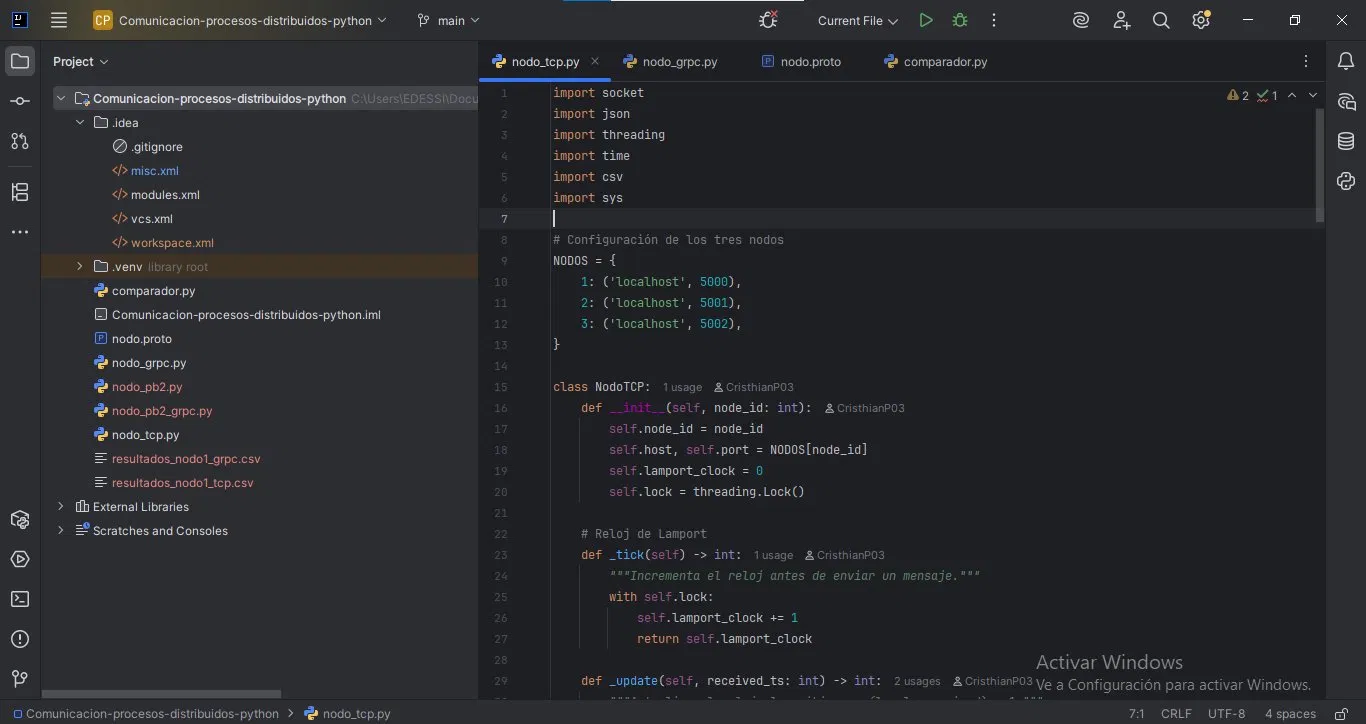
\includegraphics[width=\textwidth]{figura1_estructura.png}
    \caption{Estructura del proyecto en IntelliJ IDEA}
    \label{fig:estructura}
\end{figure}


\section{Implementación con Sockets TCP}

La implementación TCP se realizó en \texttt{nodo\_tcp.py}. Al ejecutarlo con el argumento 1, 2 o 3, el proceso abre un servidor en el puerto correspondiente (5000, 5001 o 5002) y puede también actuar como cliente enviando mensajes a los otros nodos.

Cada nodo mantiene un reloj de Lamport protegido por un \texttt{threading.Lock()} para evitar errores de concurrencia. Los dos métodos centrales del reloj son los siguientes

\newpage

\begin{lstlisting}
def _tick(self):
    with self.lock:
        self.lamport_clock += 1
        return self.lamport_clock

def _update(self, received_ts):
    with self.lock:
        self.lamport_clock = max(
            self.lamport_clock, received_ts
        ) + 1
        return self.lamport_clock
\end{lstlisting}

El servidor corre en un hilo en segundo plano. Al recibir un mensaje JSON, extrae el \texttt{timestamp} del emisor, actualiza el reloj con \texttt{\_update()} y responde con su propio timestamp actualizado. El cliente llama a \texttt{\_tick()} antes de enviar, construye el JSON y abre la conexión TCP al nodo destino. La medición de latencia se realizó sobre 100 envíos usando \texttt{time.perf\_counter()}, y los resultados se guardan en \texttt{resultados\_nodo1\_tcp.csv}.


\section{Implementación con gRPC y Protocol Buffers}

\subsection{Definición del contrato en nodo.proto}

El primer paso fue definir el servicio en el archivo \texttt{nodo.proto}, que especifica los mensajes intercambiados y el método disponible:

\begin{lstlisting}[language={}]
syntax = "proto3";

service NodoService {
  rpc Enviar (Mensaje) returns (Respuesta);
}

message Mensaje {
  string sender    = 1;
  int64  timestamp = 2;
  string message   = 3;
}

message Respuesta {
  string responder = 1;
  int64  timestamp = 2;
}
\end{lstlisting}

\subsection{Servidor y cliente gRPC}

La implementación en \texttt{nodo\_grpc.py} sigue la misma lógica de Lamport que TCP. El servidor hereda de \texttt{NodoServiceServicer} y sobrescribe el método \texttt{Enviar()}, que recibe el mensaje, actualiza el reloj y devuelve la respuesta. El cliente abre un canal hacia el nodo destino, obtiene un \textit{stub} y llama al método remoto como si fuera local, sin manejar directamente sockets ni serialización.

La principal diferencia con TCP es que gRPC delega toda la comunicación al framework, simplificando el código. Los puertos usados para gRPC fueron 6000, 6001 y 6002, distintos a los de TCP para evitar conflictos.


\section{Módulo Comparador}

Para analizar y comparar los resultados de ambas implementaciones, se desarrolló \texttt{comparador.py}. Este módulo lee los dos archivos CSV generados y calcula el promedio, mínimo y máximo de latencia de cada protocolo, mostrando al final cuál fue el más rápido. Su ejecución es independiente de los nodos y solo requiere que los archivos CSV existan previamente.

\section{Proceso de Ejecución}

Para ejecutar cualquiera de las dos implementaciones, se abren tres terminales simultáneas y se inician primero los nodos 2 y 3, ya que el nodo 1 espera 3 segundos automáticamente antes de comenzar. Una vez listos, el Nodo 1 ejecuta los 20 intercambios con reloj de Lamport, luego los 100 envíos de latencia y finalmente genera el archivo CSV.

La Figura~\ref{fig:ejecucion_tcp} muestra la salida de la terminal durante la ejecución TCP, donde se puede observar el avance del reloj de Lamport en cada intercambio, alcanzando un valor de 60 al finalizar los 20 intercambios, y la latencia promedio obtenida de 2.6357 ms.

\begin{figure}[H]
    \centering
    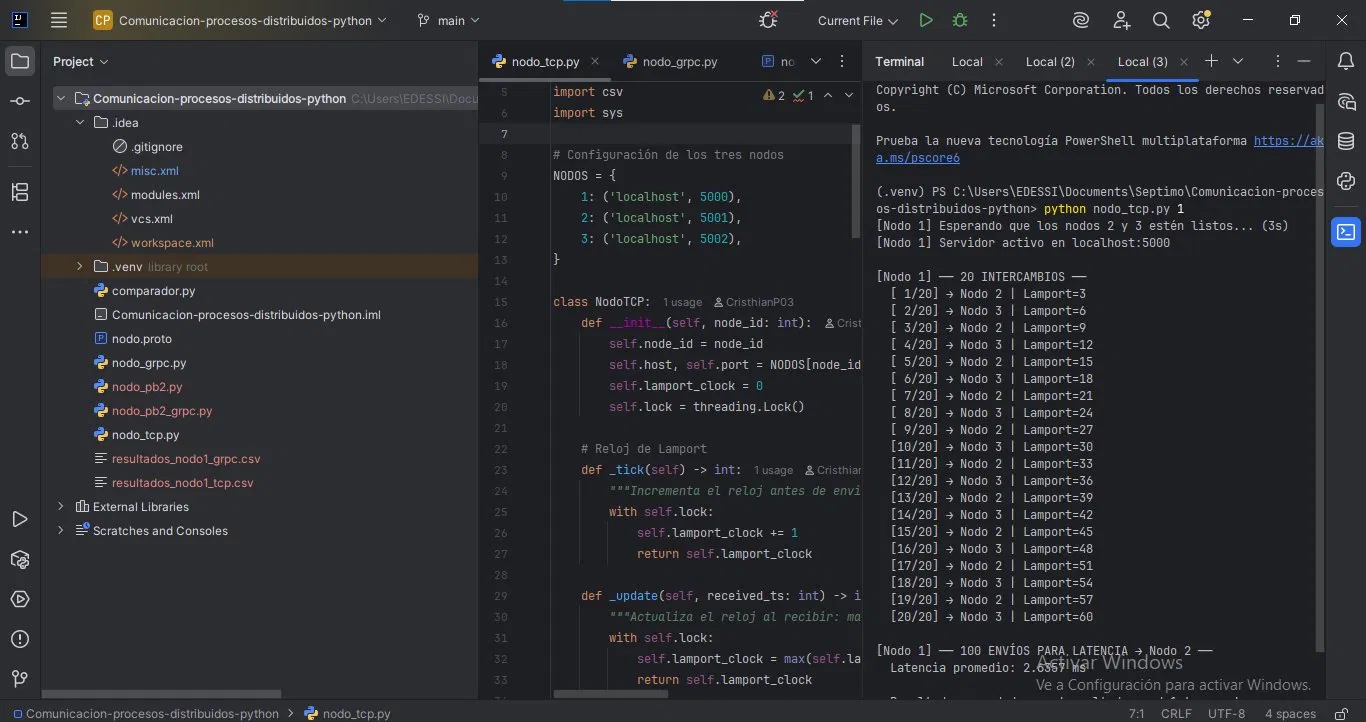
\includegraphics[width=\textwidth]{figura2_ejecucion_tcp.png}
    \caption{Ejecución de los 20 intercambios TCP con reloj de Lamport}
    \label{fig:ejecucion_tcp}
\end{figure}

De manera similar, la Figura~\ref{fig:ejecucion_grpc} muestra la ejecución del protocolo gRPC, con el mismo patrón de intercambios y una latencia promedio de 5.4692 ms.

\begin{figure}[H]
    \centering
    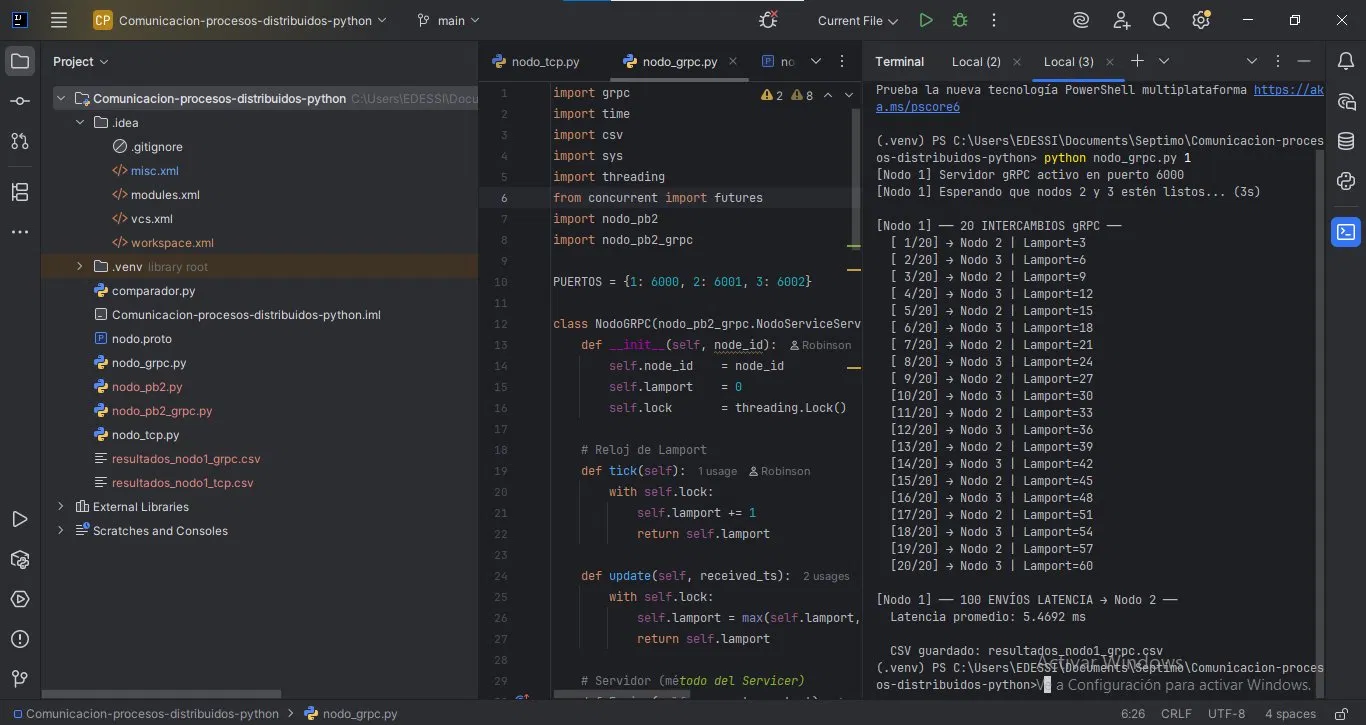
\includegraphics[width=\textwidth]{figura3_ejecucion_grpc.png}
    \caption{Ejecución de los 20 intercambios gRPC con reloj de Lamport}
    \label{fig:ejecucion_grpc}
\end{figure}

\section{Resultados}

\subsection{Comportamiento del reloj de Lamport}

En ambas implementaciones, el reloj de Lamport avanzó correctamente durante los 20 intercambios. Cada mensaje enviado incrementaba el reloj del emisor, y al recibirlo, el receptor aplicaba la regla \(\max(\text{local}, \text{recibido}) + 1\), asegurando un orden coherente de los eventos. En ambos protocolos el reloj alcanzó el valor 60 al finalizar los 20 intercambios, lo que confirma el correcto funcionamiento del algoritmo.

\subsection{Latencias obtenidas con TCP}

Los resultados de la medición de latencia TCP se almacenaron en el archivo \texttt{resultados\_nodo1\_tcp.csv}, cuyo contenido se puede observar en la Figura~\ref{fig:csv_tcp}. Los valores obtenidos fueron los siguientes:

\begin{itemize}[leftmargin=2cm]
    \item \textbf{Promedio:} 2.6357 ms
    \item \textbf{Mínimo:} 1.5026 ms
    \item \textbf{Máximo:} 13.2911 ms
\end{itemize}

\begin{figure}[H]
    \centering
    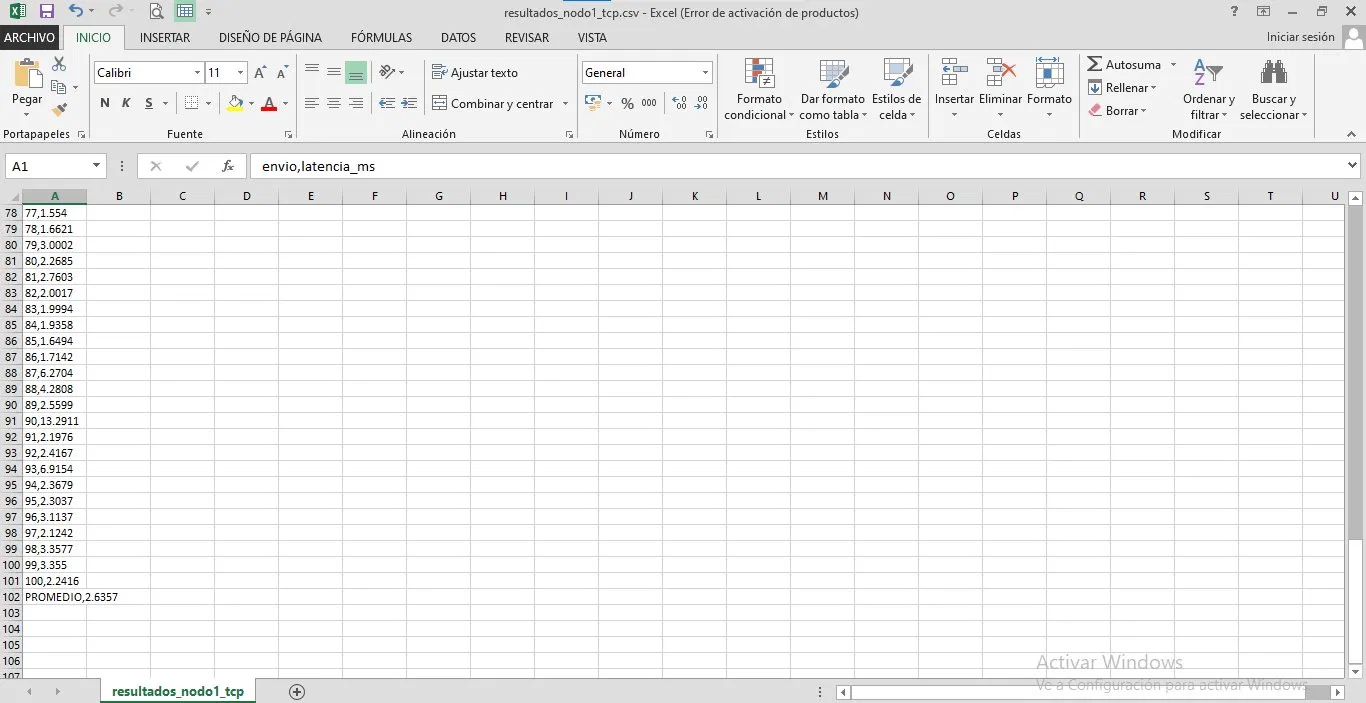
\includegraphics[width=0.75\textwidth]{figura4_csv_tcp.png}
    \caption{Archivo CSV con las latencias de los 100 envíos TCP}
    \label{fig:csv_tcp}
\end{figure}

\subsection{Latencias obtenidas con gRPC}

Los resultados de la medición de latencia gRPC se almacenaron en el archivo \texttt{resultados\_nodo1\_grpc.csv}, cuyo contenido se puede observar en la Figura~\ref{fig:csv_grpc}. Los valores obtenidos fueron los siguientes:

\begin{itemize}[leftmargin=2cm]
    \item \textbf{Promedio:} 5.4692 ms
    \item \textbf{Mínimo:} 3.3481 ms
    \item \textbf{Máximo:} 18.8438 ms
\end{itemize}

\begin{figure}[H]
    \centering
    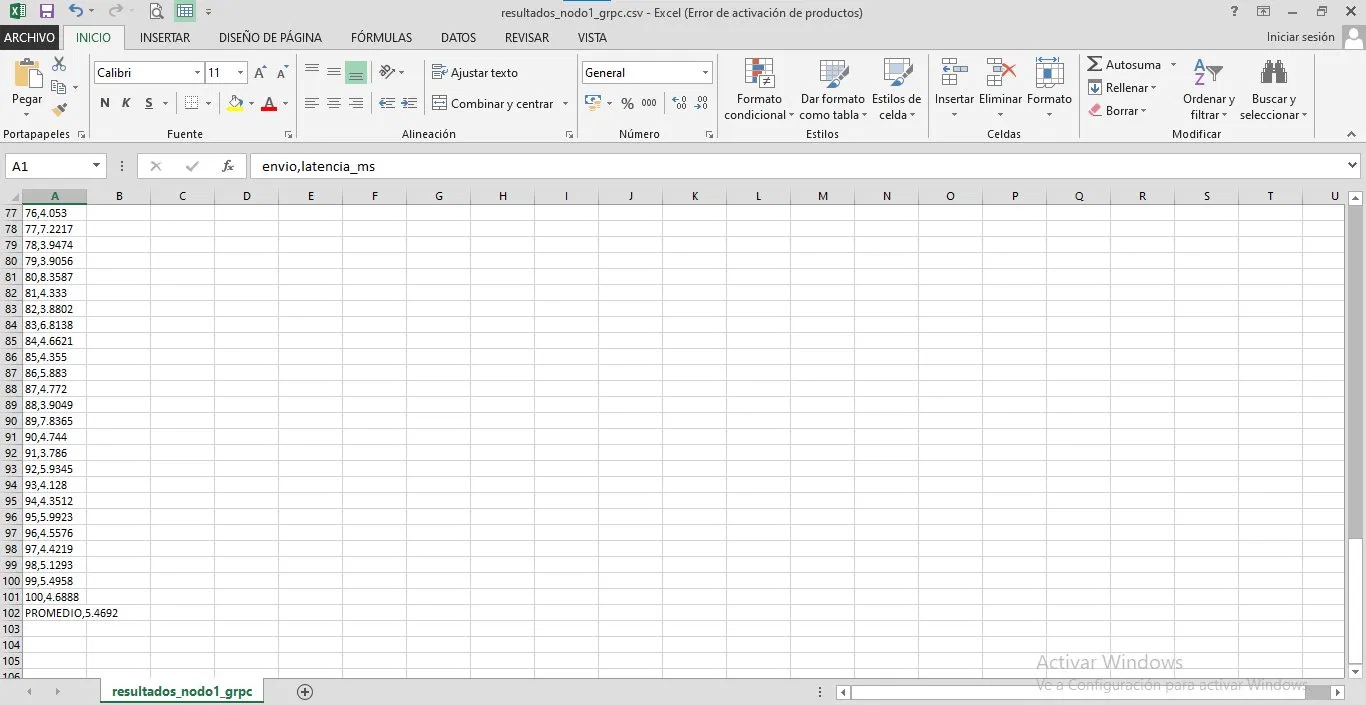
\includegraphics[width=0.75\textwidth]{figura5_csv_grpc.png}
    \caption{Archivo CSV con las latencias de los 100 envíos gRPC}
    \label{fig:csv_grpc}
\end{figure}


\section{Análisis de Resultados}

\subsection{Comparación de latencias}

La Figura~\ref{fig:comparador} muestra la salida del módulo comparador, que resume los resultados de ambos protocolos. TCP obtuvo una latencia promedio de 2.6357 ms frente a los 5.4692 ms de gRPC, siendo TCP aproximadamente dos veces más rápido en este entorno de prueba.

\begin{figure}[H]
    \centering
    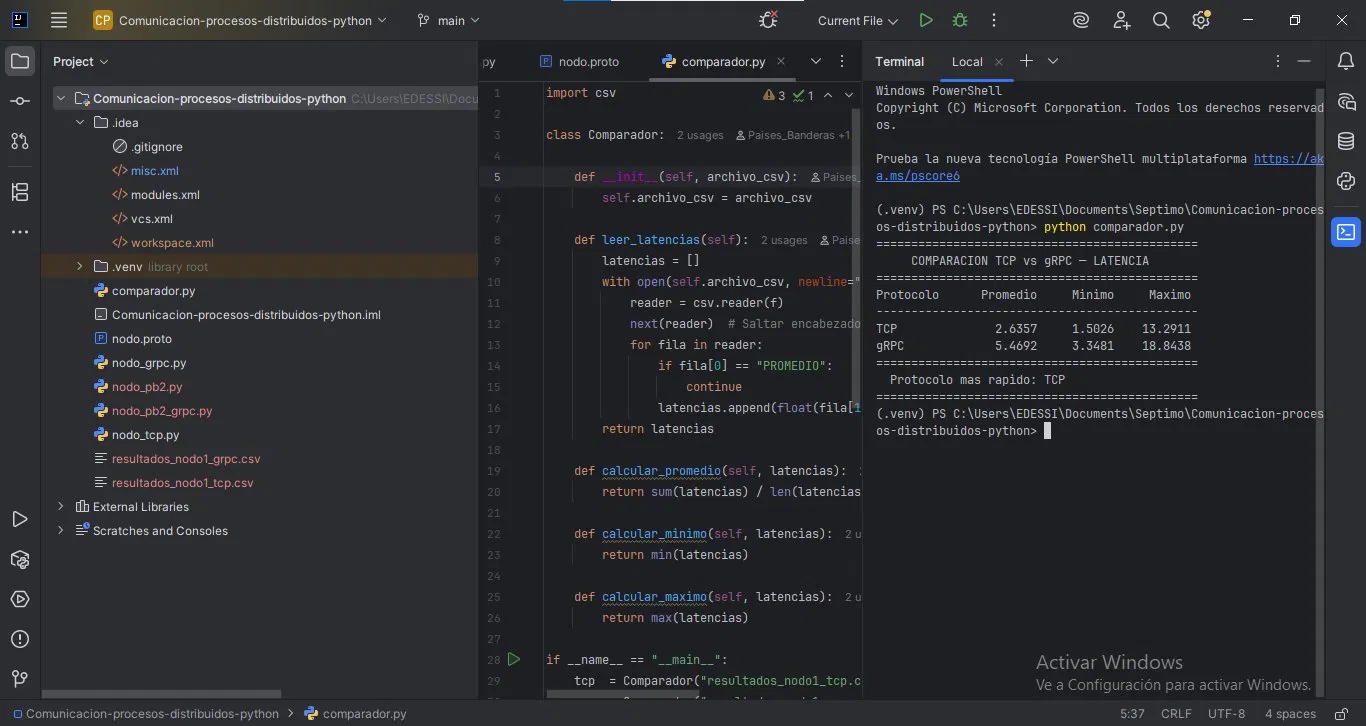
\includegraphics[width=\textwidth]{figura6_comparador.png}
    \caption{Resultado del comparador mostrando TCP vs gRPC}
    \label{fig:comparador}
\end{figure}

Esta diferencia puede explicarse porque en un entorno local, la sobrecarga de gRPC al establecer canales HTTP/2 y serializar los datos con Protocol Buffers resulta mayor que la simple apertura de un socket TCP con un mensaje JSON pequeño. En sistemas distribuidos reales con mayor volumen de datos o mayor latencia de red, los Protocol Buffers podrían ofrecer una ventaja al ser más compactos que el JSON, lo que podría invertir estos resultados \cite{niswar2024}.

\subsection{Funcionamiento del reloj de Lamport}

El reloj de Lamport funcionó correctamente en ambas implementaciones. Se verificó que en cada intercambio el valor del reloj aumentaba de forma coherente aplicando la regla \(\max(\text{local}, \text{recibido}) + 1\). En los 20 intercambios, el reloj avanzó de 0 a 60 en ambos protocolos, lo cual es consistente con lo propuesto originalmente por Lamport \cite{lamport1978}: cada envío y cada recepción generan un incremento, lo que garantiza el orden parcial de los eventos.

\subsection{Facilidad de implementación}

Desde el punto de vista del desarrollo, los Sockets TCP requieren manejar manualmente la serialización de mensajes, la apertura y cierre de conexiones, y los posibles errores de red. gRPC abstrae todos estos detalles al generar el código de comunicación automáticamente desde el archivo \texttt{.proto}. Como señalan Fu y Cai \cite{fu2019}, la complejidad de la comunicación entre procesos impacta directamente en la calidad y mantenibilidad del software distribuido. Como señala Birman \cite{birman2012}, la latencia es uno de los factores más críticos en el diseño de sistemas distribuidos confiables.


\section{Repositorio en GitHub}

El código fuente completo de esta práctica se encuentra disponible en:
 \url{https://github.com/CristhianP03/Actividades-Grupales-App-Distribuidas.git}

\vspace{0.25cm}
Las contribuciones se distribuyeron de la siguiente manera:

\begin{itemize}[leftmargin=2cm]
    \item \textbf{Cristhian Pacheco}: configuración del proyecto y \texttt{nodo.proto}, servidor TCP con parser JSON, integración del reloj de Lamport en \texttt{nodo\_tcp.py}.
    \item \textbf{Robinson Cando}: servidor gRPC con \texttt{NodoServiceImpl}, cliente gRPC con \texttt{send\_to()}, métodos de intercambio y latencia en \texttt{nodo\_grpc.py}.
    \item \textbf{Ernesto Luna}: módulo comparador con lectura de CSV, métodos de cálculo estadístico, análisis comparativo final.
\end{itemize}


\newpage
\section{Conclusiones Generales}

A través de esta práctica se implementaron y compararon dos mecanismos de comunicación en un sistema distribuido de tres nodos. Los resultados muestran que en un entorno local, TCP obtuvo una latencia promedio de 2.6357 ms, menor que los 5.4692 ms registrados por gRPC, siendo TCP el protocolo más rápido en esta prueba.

El reloj lógico de Lamport funcionó correctamente en ambas implementaciones, avanzando de forma coherente de 0 a 60 durante los 20 intercambios, lo que confirma el correcto ordenamiento de los eventos en el sistema distribuido.

Desde el punto de vista del desarrollo, gRPC ofrece mayor facilidad de implementación y mantenimiento al generar el código de comunicación automáticamente, aunque su configuración inicial es más compleja. Los Sockets TCP brindan mayor control y menor sobrecarga en entornos locales con mensajes pequeños.
\newpage
\vspace{0.5cm}
\subsection*{Conclusiones Individuales}

\textbf{Cristhian Pacheco} \\
Antes de realizar esta práctica, al momento de tener que configurar el proyecto, tener que definir el archivo \texttt{nodo.proto} y realizar la implementación del archivo del servidor TCP, me di cuenta de que detrás de cada mensaje que viaja entre los procesos hay muchas decisiones que se van a tomar: desde cómo formatear los datos, cómo abrir las conexiones hasta como tener que cerrar estas mismas, y cómo asegurarse de que los eventos ocurran en el orden correcto. Una de las cosas que más me llamó la atención fue el reloj de Lamport. Al principio me parecía una idea algo complicada, pero cuando lo implementé y vi cómo el número subía en cada intercambio que se iba realizando, entendí que es una solución a un problema real. Los resultados también me hicieron reflexionar, porque pensaba que gRPC podría llegar a ser más rápido que TCP, y no fue así al final.

\vspace{0.5cm}
\textbf{Robinson Cando} \\
Al momento de tener que realizar la implementación del archivo gRPC, al principio no entendía bien por qué razón había que definir un archivo \texttt{.proto} antes de escribir cualquier código, pero luego me di cuenta que ese archivo es como un contrato: le dice a todos los participantes del sistema exactamente qué mensajes van a enviarse y qué van a responder. Eso hace que el código sea más ordenado y menos propenso a errores. Lo que más me sorprendió fue que, a pesar de toda esa estructura, gRPC terminó siendo más lento que TCP en nuestra prueba. Después de investigar un poco, me di cuenta que esa sobrecarga existe porque gRPC hace muchas cosas internamente para garantizar compatibilidad y eficiencia en redes reales. En un escenario con más datos o más nodos, probablemente los resultados serían distintos. Esta práctica me recordó que ninguna tecnología es mejor en todos los contextos.

\vspace{0.5cm}
\textbf{Ernesto Luna} \\
La parte que me asignaron a mi fue la de construir el comparador y analizar los datos que se generaron en los otros dos módulos. Parece una tarea sencilla, pero me obligó a entender bien cómo funcionaban tanto TCP como gRPC, porque si yo no entendía cómo estaban estructurados los CSV, no podía procesarlos correctamente. Algo que me pareció interesante fue el ver que la latencia no es un número fijo: en el CSV hay envíos que tardaron 1.5 ms y otros que tardaron más de 13 ms, dependiendo de lo que estuviera haciendo el sistema en ese momento. Por eso medir el promedio de los 100 envíos es más dificil que medir uno solo. También aprendí mucho del trabajo en equipo usando GitHub. Coordinar commits con mis compañeros, revisar lo que cada uno aportó y mantener el código organizado es algo que suena fácil pero requiere disciplina. 

% ══ BIBLIOGRAFÍA 
\newpage
\begin{thebibliography}{99}

\bibitem{lamport1978}
L. Lamport, ``Time, clocks, and the ordering of events in a distributed system,''
\textit{Communications of the ACM}, vol. 21, no. 7, pp. 558--565, Jul. 1978,
doi: 10.1145/359545.359563.

\bibitem{fu2019}
X. Fu and H. Cai, ``Measuring interprocess communications in distributed systems,''
in \textit{Proc. IEEE/ACM 27th Int. Conf. Program Comprehension (ICPC)},
Montreal, QC, Canada, 2019, pp. 323--334,
doi: 10.1109/ICPC.2019.00051.

\bibitem{chamas2017}
C. L. Chamas, D. Cordeiro, and M. M. Eler,
``Comparing REST, SOAP, Socket and gRPC in computation offloading of mobile
applications: An energy cost analysis,''
in \textit{Proc. IEEE 9th Latin-American Conf. Commun. (LATINCOM)},
Guatemala City, Guatemala, Nov. 2017, pp. 1--6,
doi: 10.1109/LATINCOM.2017.8240185.

\bibitem{niswar2024}
M. Niswar, R. A. Safruddin, A. Bustamin, and I. Aswad,
``Performance evaluation of microservices communication with REST, GraphQL,
and gRPC,''
\textit{Int. J. Electron. Telecommun.}, vol. 70, no. 2, pp. 429--436,
Jun. 2024, doi: 10.24425/ijet.2024.149562.

\bibitem{vansteen2017}
M. van Steen and A. S. Tanenbaum,
\textit{Distributed Systems}, 3rd ed.
CreateSpace Independent Publishing Platform, 2017,
ISBN: 978-1-543057-38-6.

\bibitem{birman2012}
K. Birman,
\textit{Guide to Reliable Distributed Systems: Building High-Assurance
Applications and Cloud-Hosted Services}.
New York, NY, USA: Springer, 2012,
doi: 10.1007/978-1-4471-2416-0.

\end{thebibliography}

\end{document}
